\chapter{Chaos in theory and experiments}
\label{chap: chaos}

\section{Dynamical systems}
\label{sec: dynamical systems}

The concept of dynamical systems is quite general, since anything that moves can be considered as a
dynamical system~\cite{ref:fractal_dim}. If these changes are driven
by specific rules, we say that the system is deterministic; otherwise, if the rules
are random, it is stochastic. The main feature of chaotic systems is the fact that they are unpredictable
despite being deterministic; in order to better explain the meaning of this statement, it is essential
to involve some mathemathical definitions.

The instantaneous state of a dynamical system is described by a vector $\mathbf{s}$ within a
state space $\mathcal{S}$ (typically, $\mathcal{S}\subseteq \mathbb{R}^M$).
The state vector evolves in time according to an evolution operator $\mathcal{E}_t$ such that:
\begin{equation}
\label{eq: state space evolution}
    \mathbf{s}(t+t_0)=\mathcal{E}_t[\mathbf{s}(t_0)].
\end{equation}

In theoretical systems the state space $\mathcal{S}$ is well-defined and the evolution operator
$\mathcal{E}_t$ is given; in most cases, $\mathcal{E}_t$ is defined by a set of differential equations
which can be solved, analytically or numerically, to find the system's evolution $\mathbf{s}(t)$
out of the initial conditions $\mathbf{s}(0)$.

A dynamical system is defined to be linear if the superposition principle holds, i.e.:
\begin{equation}
\label{eq: linear systems}
    \mathcal{E}_t[c_1\mathbf{s}_1+c_2\mathbf{s_2}]=c_1\mathcal{E}_t[\mathbf{s}_1]+
    c_2\mathcal{E}_t[\mathbf{s}_2].
\end{equation}
If the last equality is not satisfied the system is said to be nonlinear.
Nonlinearity is a necessary (but not sufficient) condition for the system to be chaotic.

In experimentally observed systems the state space is not always fully accessible; moreover,
the evolution operator $\mathcal{E}_t$ is rarely known.
Observing a system consists in recording some signal $y(t)$ out of it through some measurement
function $\mathcal{M}$ acting on the system's state, i.e. $y(t)=\mathcal{M}[\mathbf{s}(t)]$.
This continuous signal is always sampled and digitized, producing a finite time series (or sequence)
$\{y_n\}$ with $n=1,...,\ell$.


\section{Formal definition of chaos}
\label{sec: chaos in theory}

An universally accepted mathematical definition of chaos does not exists but
a commonly used definition is the following, originally formulated by Robert L.
Devaney~\cite{ref:chaos_definition}.

Three conditions are necessary and
sufficient to define a system as chaotic: (i) sensitivity to initial conditions;
(ii) topological transitivity;
(iii) density of periodic orbits.

Going into detail:
\begin{itemize}
    \item[(i)] Sensitivity to initial conditions is a property that characterizes chaotic
    systems and makes their evolution hard to predict.

    Given two initial conditions $\mathbf{s}_1(0)$, $\mathbf{s}_2(0)$ that are arbitrarily close within the state
    space ($||\mathbf{s}_1(0)-\mathbf{s}_2(0)||<\varepsilon$),
    the system having sensitive dependence on initial conditions means that
    the two trajectories evolving out of these initial conditions diverge exponentially in time, i.e.
    for large $t$:
    \begin{equation}
    \label{eq: trajectory divergence}
        ||\mathbf{s}_1(t)-\mathbf{s}_2(t)||\propto e^{\lambda t},
    \end{equation}
    where $\lambda$ is called maximum Lyapunov exponent (MLE).
    In order for the system to be chaotic, $\lambda$ has to be positive.

    It is also important that the orbits $\mathbf{s}_1(t)$, $\mathbf{s}_2(t)$ remain bounded at large $t$,
    otherwise, if orbits went to infinity, it would be simple for their distance to diverge exponentially.
    
    The most important consequence of this property is that, as far as we are
    able to precisely measure the initial state of a system, there will always be
    a small error (given for example by measuring instruments) which can grow
    rapidly over time. Therefore, even if we know exactly the deterministic laws
    governing time evolution, our predictions on the behaviour of the system
    after a certain time will no longer be reliable. Furthermore, if the precision
    with which we measure the state of the system in the initial instant is
    improved by a factor of $10$, we only gain a $\log(10)$ factor for the maximum
    time for which the predictions are accurate.

    \item[(ii)] Topological transitivity is the property according to which a chaotic trajectory eventually connects
    any region of the state space with any other. In other words, the state space of a chaotic system
    cannot be decomposed into disjoint subsets.

    \item[(iii)] Density of periodic orbits means that for any given point in the state space
    there is a periodic orbit that passes arbitrarily close to it, i.e. periodic orbits make up a dense set.

\end{itemize}


\section{The issue of detecting chaos}
\label{sec: chaos in experiments}

When dealing with experimentally observed systems, the precise laws that describe the dynamics are unknown.
What is known is the time series, which can be used to assess condition (i) of Devaney's definition
of chaos. Instead, conditions (ii) and (iii) are difficult to identify with the time series only.
However, there are observable consequences. In particular, the time
evolution of a chaotic system in the state space always converges to an object called strange
attractor, characterized by a fractal structure~\cite{ref:fractal_dim,ref:fractal_book}.
An example can be seen in Fig.~\ref{fig: lorenz attractor}.
This means that strange
attractors exhibit self-similarity (or self-affinity\footnote{In general, it is more correct to speak
of self-affinity, since in the case of self-similarity the
object is scaled by the same amount in all space directions, but in self-affinity scaling is not
necessary identical in all directions~\cite{ref:mandelbrot_fractal}.}) and have a non-integer dimensionality.

\begin{figure}[h!]
\centering
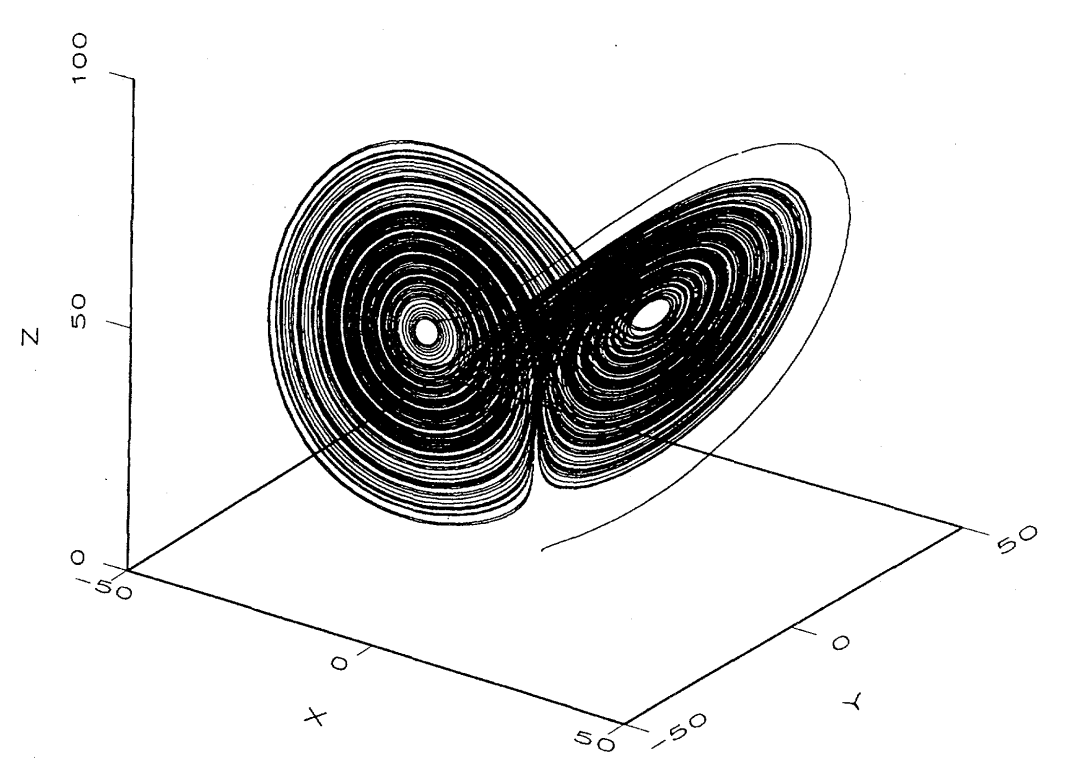
\includegraphics[width=.6\linewidth]{images/lorenz_attractor.png}
\caption{
    Lorenz attractor~\cite{lorenz1963deterministic} in three-dimensional phase space
    $(x(t),y(t),z(t))$. Figure adapted from Ref.~\cite{ref:abarbanel_fourier_spectra}.
}\label{fig: lorenz attractor}
\end{figure}

To understand what it means to have non-integer dimensionality, suppose
to consider a fractal object with dimension $1 < D < 2$.
We know in general that if we have an object of dimension $D$ (assuming that
it has a mass density), taking an arbitrary point in it and considering an open
ball centered in that point, we can measure the mass contained in the ball as
a function of the radius. For small distances $m(r)\propto r^D$. For the same density
and radius, the fractal ``weighs" more than a line but less then a surface, as if
a dense set (which is the set of the periodic points) had been removed from the
surface.

Self-similarity, instead, is the exhibition of similar patterns at increasingly smaller
scales; in other words, a fractal does not appear simplified when we see it zoomed,
as can be seen in Fig.~\ref{fig: henon fractal}. Despite strange attractors
also existing in non-chaotic systems~\cite{ref:strange_attractors_non_chaotic}, the estimate of the system's non-integer dimension
is often used as a tool to identify chaos.

\begin{figure}[h!]
    \centering
    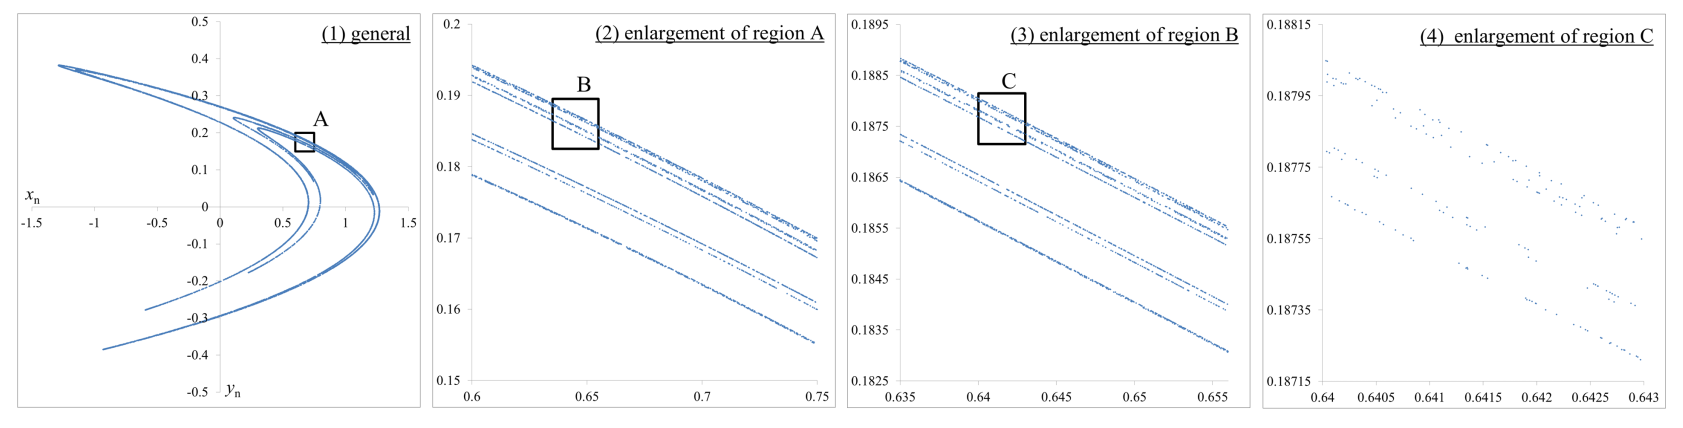
\includegraphics[width=\linewidth]{images/henon_fractal.png}
    \caption{Self-similarity of the Henon attractor: at all magnification levels the same
    qualitative structures are visible. Figure adapted from Ref.~\cite{henon2004two}.}
    \label{fig: henon fractal}
\end{figure}

Another important property allows
us to identify chaos: the trajectory winds around forever never repeating on a
strange attractor and the time series arising by chaotic systems are aperiodic
and characterized by broad, noise-like Fourier spectra, as can be seen in Fig.~\ref{fig: lorenz spectrum}.
This also means that linear techniques
such as fast Fourier transform (FFT) applied to sequences cannot distinguish between a chaotic system
and a stochastic one, e.g. a Gaussian white noise source (GWN).

\begin{figure}[h!]
    \centering
    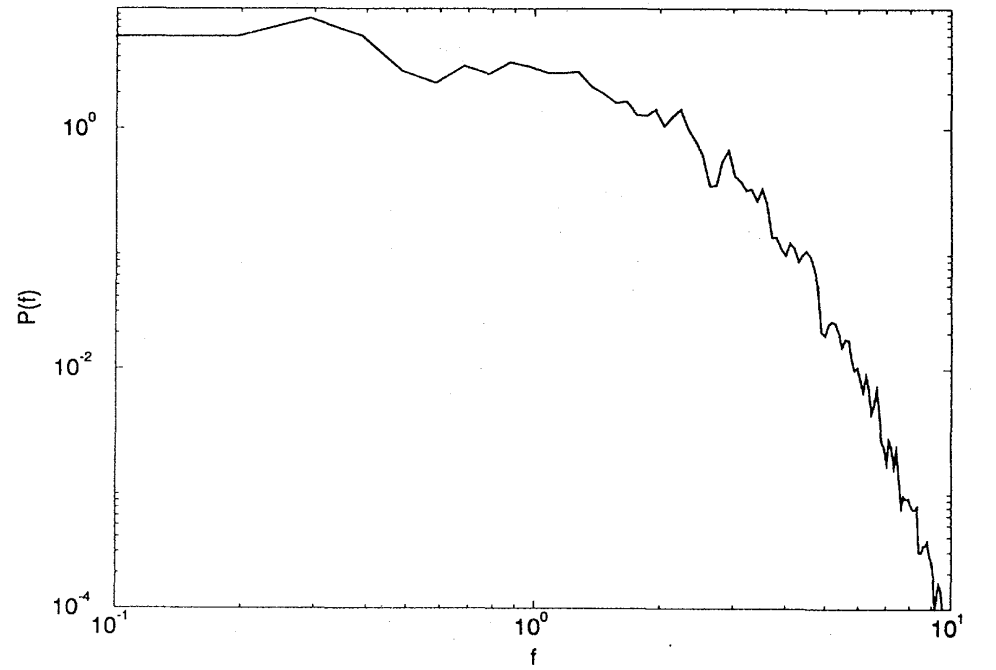
\includegraphics[width=.6\linewidth]{images/lorenz_spectrum.png}
    \caption{
        Power spectrum of the Lorenz system~\cite{lorenz1963deterministic}.
        Figure adapted from Ref.~\cite{ref:abarbanel_fourier_spectra}.
    }\label{fig: lorenz spectrum}
\end{figure}

One more necessary requirement to sustain a chaotic flow is that
the number of independent dimensions has to be at least three, assuming no discontinuities~\cite{ref:chaos_two_dim_theorem};
this is due to the fact that
with two or less independent variables the trajectory will eventually intersect itself, which
cannot happen due to the aperiodic nature of chaotic dynamics.


\section{The embedding procedure}
\label{sec: embedding}

In experimentally observed systems it is only possible to utilize the finite time series $\{y_n\}$,
with the aim to at least obtain some invariant quantities, e.g. the maximum Lyapunov exponent or
the ``effective" dimension of the system. Under certain conditions, a procedure exists with which
it is possible to reconstruct the entire state space using only one variable, which is a
function of the state space vector $\mathbf{s}(t)$. This procedure is called ``time delay embedding''
\cite{ref:packard1980geometry}.

Embedding consists in building a sequence of $m$-dimensional vectors $\mathbf{Y}_n$ by picking
$m$ time-delayed samples of the sequence $y_n$, i.e.:
\begin{equation}
    \label{eq: embedding}
    \mathbf{Y}_n=\left(y_n,y_{n+L},y_{n+2L},...,y_{n+(m-1)L}\right),
\end{equation}
where the parameter $L$ is an integer number and is called ``lag''. It is perfectly equivalent to make use of
a ``causal'' version of Eq.~\ref{eq: embedding} in which the chosen samples are $y_{n-kL}$ instead of
$y_{n+kL}$, with $k=0,\ldots,m-1$~\cite{ref:bradley2015nonlinear}.

An example of embedding can be seen in Fig.~\ref{fig: rossler embedding}.
This procedure maps the time series into a ``reconstructed space'' in which the trajectory
somehow resembles a strange attractor.

\begin{figure}[h!]
    \centering
    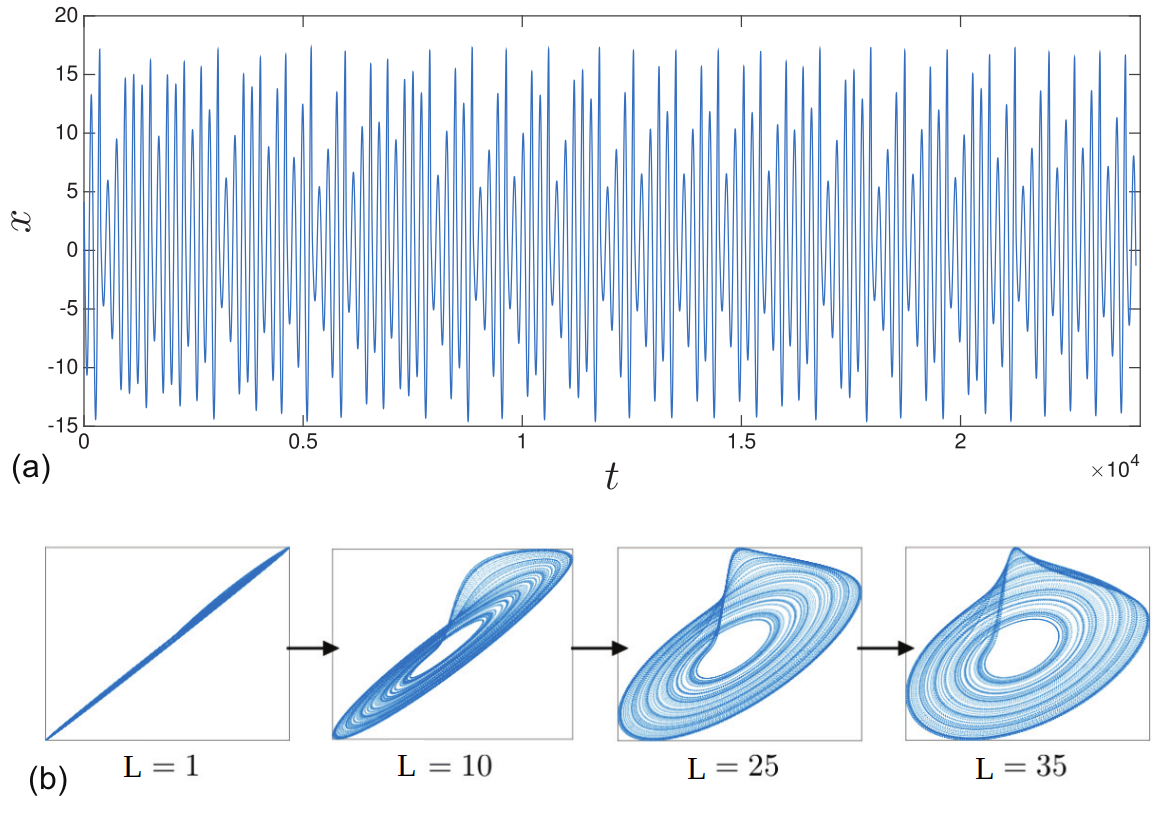
\includegraphics[width=\linewidth]{images/rossler_embedding.png}
    \caption{
    A time series from the Rossler system (a)~\cite{rossler1977continuous}
    and a number of delay-coordinate embeddings of that time series with different values of the lag $L$ (b).
    Figure adapted from Ref.~\cite{ref:bradley2015nonlinear}.}\label{fig: rossler embedding}
\end{figure}

It has in fact been proven by Takens~\cite{ref:takens2006detecting} and Ma{\~n}{\'e}~\cite{ref:mane2006dimension} that
if the parameters $m$ (dimension) and $L$ (lag) are suitably chosen,
the reconstructed state space evolution is topologically identical to the actual state space dynamics.
This means that a ``good” embedding provides a smooth one-to-one map from the
original state space evolution to the reconstructed one, therefore enabling us to estimate the
properties of the original system that are invariant under this mapping.

The two conditions under which Takens' theorem holds regard the embedding parameters $(m,L)$.
The first one requires that $m>2D$, where $D$ is the dimension of the manifold corresponding to the
time evolution of the system, which is not known a priori; this condition can be relaxed to $m>D$ if
estimating correlation dimension~\cite{ref:ding1993estimating}.
The second one states that $L$ is not a multiple of the period of any system's orbit~\cite{ref:grassberger1991nonlinear}.

Aside from these two minimal conditions, since Takens' theorem is an existence theorem, it does not
give any hint on how to find the best embedding parameters. The reason for this is that as long as the
two conditions are met, every choice for the couple $(m,L)$ is good for reconstruct the dynamics;
however, this is valid only for noiseless, finely sampled and infinitely long sequences. In reality,
the issue of optimal embedding is a very active field in the physics of chaos, and several techniques
have been developed in order to overcome this problem~\cite{ref:perinelli2018identification,ref:perinelli2020chasing,ref:casdagli1991state}.

%m PROBLEMS
Considering the dimension $m$, choosing $m\gg1$ ensures, in principle, that $m$ is
greater than $2D$. However, if $m$ is too large the directions orthogonal to the deterministic noiseless
trajectory will be dominated by noise and will not provide extra information; in other words, supposing
that $m_0$ is the minimum dimension for which the system is correctly embedded, the remaining $m-m_0$
dimensions would be populated by noise, being thus redundant and resulting in an increase of the
computational cost. Moreover, the larger is the embedding dimension $m$,
the fewer independent embedding vectors are available, which is an issue considering the finiteness
of the time series.

%L PROBLEMS
The choice on the lag $L$ is also not trivial. If $L$ is too short, the elements of the embedding vectors
$\mathbf{Y}_n$ will be strongly correlated, resulting in all the points being clustered on the
diagonal of the reconstructed space (see Fig.~\ref{fig: rossler embedding}b);
in presence of noise, therefore, the trajectory would be
indistinguishable from the diagonal itself. On the other hand, a too large $L$ presents the opposite
problem, i.e. the elements of $\mathbf{Y}_n$ to be completely uncorrelated with each other;
this implies that the time evolution is ``blurred'', in the sense that the trajectory is folded over on itself
and the system evolution is lost.


\subsection{The embedding lattice}
\label{subsec: embedding lattice}

Since a single optimal choice for $(m,L)$ does
not necessarily exist, the embedding of the sequence can be carried out for several values of the
embedding parameters, considering that several values for the pair
$(m, L)$ can provide reconstructions of the underlying dynamics that are equivalently good.
More specifically, the procedure is carried out for each element of an embedding lattice, i.e.
$\{(m,L)|m\in[2,m_{\max}],L\in[1,L_{\max}]\}$.

Suitable embedding choices are expected to comply with two requirements concerning the
corresponding embedding window $w=(m-1)LT$, which corresponds to the
time span covered by each embedding vector.
On the one hand, the embedding window has to be larger than the redundance time $\tau_R$, so that
the points in the reconstructed space are not too close to the diagonal, as discussed in Section
\ref{sec: embedding}. On the other hand, the embedding window has to be
smaller than the irrelevance time $\tau_I$, after which the points are causally disconnected
and the noise overcomes the dynamics.

The above requirements can then be expressed as $\tau_R/T \lesssim w \lesssim \tau_I/T$.
In the embedding lattice, each window $w$ identifies a hyperbola.
Therefore, the irrelevance and redundance times correspond to two hyperbolae
within the embedding lattice, and the region bounded by them is where suitable
embedding choices can be expected.


\section{Maximum Lyapunov exponent}
\label{sec: mle}

It is now important to formally define the invariant
quantities that will be used to decide if an experimentally observed system is chaotic or not,
the first one being the maximum Lyapunov
exponent (MLE)~\cite{ref:abarbanel_fourier_spectra,wolf1986quantifying}.
There are as many Lyapunov exponents as the number of state space dimensions: each exponent $\lambda_i$
corresponds to one of the independent directions along which fiducial volumes within the state space
contract ($\lambda_i<0$) or expand ($\lambda_i>0$) in an infinitesimal time interval.
The MLE $\lambda_1$ is the most relevant of the spectrum, since its sign establishes whether the system
stabilizes on a fixed point ($\lambda_1<0$), stablizes on a limit cycle ($\lambda_1=0$) or is unstable
($\lambda_1>0$). A positive MLE is the main hallmark of chaos.

The qualitative behavior of the Lyapunov exponents is shown in Fig.~\ref{fig: lorenz lyapunov}.
In these figures three kinds of phase-space behaviour are displayed.
In Fig.~\ref{fig: lorenz lyapunov}a an exponential divergence
of two nearby points on different orbits in the attractor is shown.
This chaotic motion is
characterised by a positive Lyapunov exponent. In Fig.~\ref{fig: lorenz lyapunov}b the
behaviour of nearby points on the same orbit in the attractor is shown. The
separation of these points neither grows nor shrinks exponentially fast so
the associated Lyapunov exponent is zero. Finally, in Fig.~\ref{fig: lorenz lyapunov}c, the
decay of a transient or perturbation to the attractor is illustrated.
The associated exponent is negative.

\begin{figure}[h!]
\centering
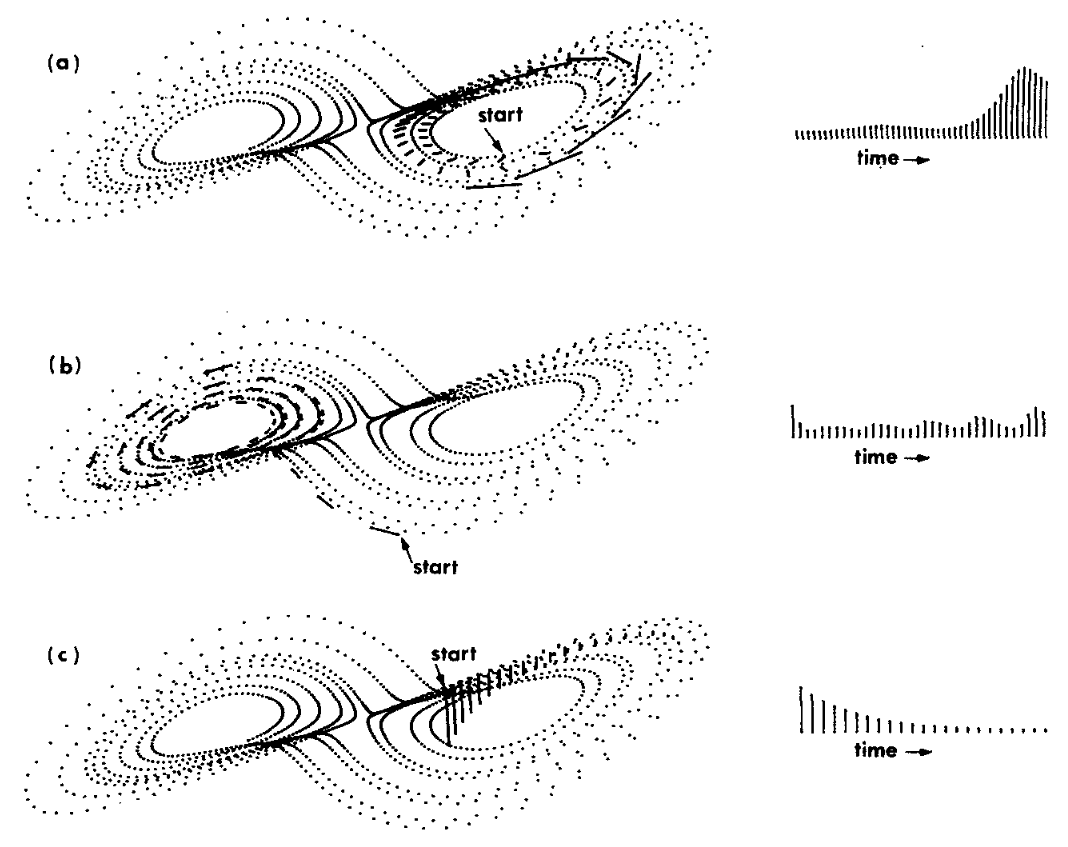
\includegraphics[width=\linewidth]{images/lorenz_lyapunov.png}   
\caption{
    Short-term evolution of the separation vector between three pairs of
    nearby points is for the Lorenz attractor \cite{lorenz1963deterministic}.
    The true magnitude of the evolving
    vector appears to the right of each figure, (a) An expanding direction ($\lambda_1>0$). (b)
    A slower than exponential direction ($\lambda_2=0$). (c) A contracting direction ($\lambda_3<0$).
    Figure adapted from Ref. \cite{wolf1986quantifying}.
}
\label{fig: lorenz lyapunov}
\end{figure}

It is possible to estimate the MLE through the embedded sequence by making use of the so-called
divergence rate method~\cite{ref:gao1993local}. This method
is based on the evaluation of the time-dependent divergence exponent $\Lambda(k)$,
which quantifies the average separation of nearby trajectories.
The estimation of this exponent is done by selecting random pairs $(i,j)$ of neighboring vectors
in the embedded sequence $\{\mathbf{Y}_n\}$, i.e. such that $||\mathbf{Y}_i-\mathbf{Y}_j||<r$,
where $r$ is some ``shell radius''; the divergence exponent is then calculated as:
\begin{equation}
    \label{eq: divergence exponent}
    \Lambda^{m,L}(k)=\frac{1}{N_{\text{pairs}}}\sum_{i,j}\log\left(
        \frac{||\mathbf{Y}_{i+k}-\mathbf{Y}_{j+k}||}{||\mathbf{Y}_i-\mathbf{Y}_j||}
    \right),
\end{equation}
where the superscript $^{m,L}$ indicates once again the dependence on the embedding parameters.

The time-dependent divergence exponent
measures the progressive separation, as a function of the time delay $k$, of the trajectories corresponding
to initially close points $\mathbf{Y}_i,\mathbf{Y}_j$.
The initial proximity of the vector pairs is tuned by changing the shell
radius $r$, which is typically estimated as the distance corresponding to the a given percentile $p$ of the
sample distribution of all Euclidean distances 
\cite{ref:franchi2014statistical,ref:ricci2020asymptotic}.

A source of error regarding the estimation of the MLE are temporal correlations within the input sequence.
This issue can be avoided by selecting pairs of points that are distant in time more than some delay
$c_0$, i.e. constraining $|i-j|\geq c_0$. Typically, $c_0$ is chosen to be the first zero of the
autocorrelation function~\cite{ref:theiler1986spurious} or its first minimum~\cite{ref:albano1995kolmogorov}.

If the underlying system is chaotic, $\Lambda(k)$ is expected to grow linearly with $k$,
as a result of the exponentially increasing numerator within the logarithm of Eq.~\ref{eq: divergence exponent}.
Suitably fitting this linear growth provides the value of the MLE.
The growth of $\Lambda(k)$ cannot continue for arbitrarily large values of $k$:
eventually, the separation becomes comparable to the size of the attractor
and the divergence exponent saturates.
This can be seen in Fig.~\ref{fig: lorenz divergence}.

\begin{figure}[h!]
\centering
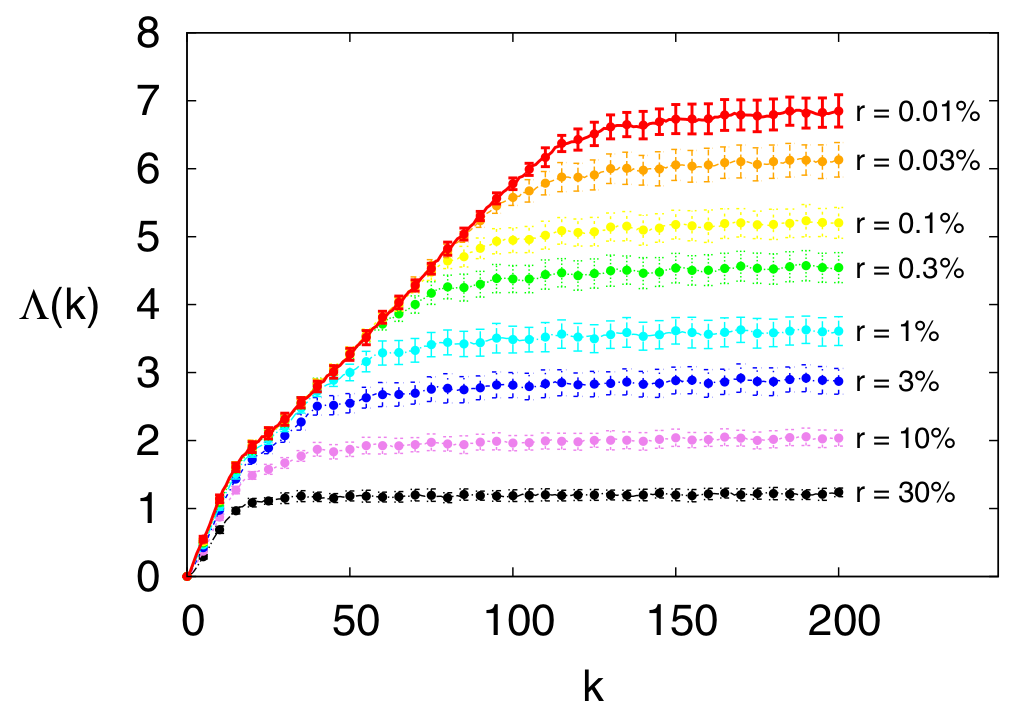
\includegraphics[width=.6\linewidth]{images/lorenz_divergence.png}
\caption{
    Time-dependent divergence exponent $\Lambda(k)$ for the Lorenz attractor \cite{lorenz1963deterministic},
    obtained by using the embedding pair
    $(3,3)$. The different plots correspond to eight different values of $r$:
    0.01\%, 0.03\%, 0.1\%, 0.3\%, 1\%, 3\%, 10\%, and 30\%. For the sake of
    clarity, only one point every five is plotted.
    Figure adapted from Ref. \cite{ref:franchi2014statistical}.
}
\label{fig: lorenz divergence}
\end{figure}


\section{Correlation dimension}
\label{sec: correlation dimension}

The second fundamental invariant quantity that characterizes a chaotic system is
the correlation dimension~\cite{ref:abarbanel_fourier_spectra}.
The simplest definition of dimension is the (integer) number of coordinates that are
needed to specify a state, e.g. the number of differential equations of a system.
This is the geometrically related to the concept of how (hyper) volumes scale as a
function of a characteristic length parameter.
One way to estimate the dimension of a set of points is the box-counting method, which consists in partitioning the space in
hypercubes of size $l$ and by counting, as a function of $l$, the fraction $\eta(l)$ of
these hypercubes containing at least one point of the set. The dimension can then be calculated
using the fact that $\eta(l\rightarrow0)\propto l^D$. Since this method is
very sensitive and computationally demanding~\cite{ref:greenside1982impracticality},
it is useful to search for other ways to estimate the dimension.

Given a set of points $\{\mathbf{Y}_n\}$ within an $m$-dimensional space partitioned in hypercubes
of size $l$, and given $p_i$
the fraction of points of the set that fall within the $i$-th hypercube,
the generalized dimension is defined as~\cite{ref:fractal_dim}:
\begin{equation}
    \label{eq: generalized dimension}
    D_q=\lim_{l\rightarrow0}\frac{1}{q-1}\frac{\log(\sum_i p_i^q)}{\log l}.
\end{equation}

This definition provides a whole spectrum of invariant quantities for $-\infty<q<\infty$.
For example, $D_0$ is exactly the dimension calculated with the box-counting method, i.e.:
\begin{equation}
    \label{eq: D_0}
    D_0=\lim_{l\rightarrow0}\frac{\log(\sum_i1)}{\log l}
    =\lim_{l\rightarrow0}\frac{\log\eta(l)}{\log l}.
\end{equation}

The dimension for $q\rightarrow1$ can instead be calculated using L'Hospital's rule, resulting in:
\begin{equation}
    \label{eq: D_1}
    D_1=\lim_{l\rightarrow0}\frac{\sum_i p_i\log p_i}{\log l}.
\end{equation}
$D_1$ is called informational dimension~\cite{ref:abarbanel_fourier_spectra} due to the numerator
being related to information entropy. In a uniform fractal, in which
$p_i=1/N$ for every $i$, $D_1=D_0$; instead, if the $p_i$ are different $D_1<D_0$.
This is true in general for every $q$, namely $D_i\leq D_j$ if $i>j$, when the equality only
holds in a uniform fractal.

Finally, one of the most utilized dimensions in chaos theory is the correlation dimension, defined as:
\begin{equation}
    \label{eq: D_2}
    D_2=\lim_{l\rightarrow0}\frac{\log(\sum_i p_i^2)}{\log l}.
\end{equation}
The numerator constitutes a two-point correlation function, measuring the probability of finding a
pair of random points within a given partition element, just as the numerator in the definition of
$D_1$ measures the probability of finding one point in a given element.

The reason why correlation dimension is so utilized lies in the fact that there is a very
efficient way to estimate it, observed by Grassberger and Procaccia~\cite{ref:grassberger1983measuring}.
Due to the exponential divergence of the trajectories, most pairs
$(\mathbf{Y}_i,\mathbf{Y}_j)$ with $i\neq j$ will be dynamically uncorrelated
pairs of essentially random points. The points lie however on the attractor, therefore they will be
spatially correlated. This spatial correlation can be measured with the correlation integral
$C(r)$, defined as:
\begin{equation}
    \label{eq: correlation integral}
    C(r) = \lim_{\ell\rightarrow\infty} \frac{1}{\ell^2}\times\left\{
        \text{number of pairs $(i,j)$ whose distance is less than $r$}
    \right\},
\end{equation}
where $\ell$ is the total number of points in the reconstructed space.
Grassberger and Procaccia proved that for small distances the correlation integral grows as
$C(r)\propto r^{D_2}$. It is thus possible to estimate the correlation dimension
by extracting random pairs of vectors in the embedded sequence, evaluating then a ``sample''
version of Eq.~\ref{eq: correlation integral}, namely:
\begin{equation}
    \label{eq: sample correlation integral}
    C^{m,L}(r)=\frac{1}{N_{\text{pairs}}}\sum_{i,j}\theta\left(
        r-||\mathbf{Y}_i-\mathbf{Y}_j||
    \right),
\end{equation}
where $\theta(x)$ is the Heaviside function and the superscript $^{m,L}$ indicates the dependence of this
sample correlation integral on the embedding parameters. 

Like in Section~\ref{sec: mle}, it is important that the time separation between
the pairs $(i,j)$ is greater than the autocorrelation time, i.e. $|i-j|\geq c_0$ 
\cite{ref:theiler1986spurious,ref:albano1995kolmogorov}.
Ignoring this issue can lead to underestimates of the dimension $D_2$~\cite{ref:theiler1986spurious}
or spurious contributions even in the case of stochastic sequences~\cite{ref:osborne1989finite}.

Another efficient manner to estimate the correlation dimension makes use of the divergence exponent
$\Lambda(k)$. As was already discussed in Section~\ref{sec: mle}, if $\Lambda(k)$ exhibits a
linear behavior it is possible to estimate the MLE as the slope of the curve.

For sufficiently large values of $k$, the divergence exponent $\Lambda(k)$
reaches a saturation value $\Lambda_{\text{pl}}$, referred to as a ``plateau" (see Fig.~\ref{fig: lorenz divergence}).
In the case of a chaotic source of finite correlation dimension $\nu$, the plateau
turns out to linearly depend on the logarithm of the percentile $p$~\cite{ref:perinelli2020chasing}:
\begin{equation}
    \label{eq: Lambda plateau}
    \Lambda_{\text{pl}}=\Lambda'-\frac{1}{\nu}\log p,
\end{equation}
where $\Lambda'$ is a constant that depends on the embedding parameters.
This dependence can thus be exploited to estimate the
sample correlation dimension $\nu$ out of an input scalar sequence by
carrying out a linear fit on a set of $(\log p, \Lambda_{\text{pl}})$ data points.


\section{The uniformity region}
\label{sec: uniformity region}

It is now possible to define a criterion that establishes whether and embedding
pair $(m,L)$ correctly reconstructs the state space or not.
A possible approach consists in searching for a so-called ``uniformity region'' in the embedding
lattice~\cite{ref:perinelli2020chasing}, i.e. a region in which the correlation dimension $\nu$
does not change significantly.

If a system having dimension $D$ is embedded with $m < D$, the full dimensionality of the system cannot
be unfolded and the embedded sequence simply fills all the available space. Consequently, for any
$m < D$, correlation integrals exhibit a scaling $\propto r^m$, rather than $\propto r^D$.
On the other hand, for $m > D$ and regardless of $m$, the correct scaling $\propto r^D$ holds in principle;
in reality, due to the presence of noise, which has infinite correlation dimension, the scaling will
be $\propto r^m$ also in the case of too large $m$ values.

This statement can also be interpreted in the following way.
If the embedding window $w$ is too small or too large, the estimated correlation dimension $\nu$
will be different from the actual dimension of the system; however, there exists an intermediate region
in which $\nu$ is the correct correlation dimension, thus $\nu$ will be practically constant in
the entirety of this region. This uniformity region is the one in which the embedding window lays between
the redundance time $\tau_R$ and the irrelevance time $\tau_I$.


\section{A method for detecting chaos}
\label{sec: method for chaos}

The most utilized tools for detecting chaos, namely the embedding lattice, the maximum Lyapunov exponent
and the correlation dimension, have now been introduced.
It is thus possible to establish an efficient procedure which not only searches for the best
embedding parameters $(m,L)$, but also provides estimates for the invariant quantities that
characterize chaos~\cite{ref:perinelli2020chasing}.

\begin{itemize}

\item
The scalar sequence $\{y_n\}$ is obtained by sampling the signal $y(t)$ with a sampling time $T$;
the time series is then supposed to be standardized as
$y \rightarrow (y - \bar{y})/\bar{\sigma}$, where $\bar{y}$ and $\bar{\sigma}$ are the sequence's
sample mean and sample standard deviation, respectively.


\item
The maximum values for the embedding dimension $m$ and lag $L$ are chosen, so that the embedding
lattice $\{(m,L)|m\in[2,m_{\max}],L\in[1,L_{\max}]\}$ is well defined.


\item
For each value of $(m,L)$ the divergence exponent $\Lambda^{m,L}(k)$ is calculated with the methods
discussed in Section~\ref{sec: mle}, and for different values of the percentile $p$.
An important step in the algorithm is that, rather than
considering a single calculation for each value of $k$, each point of $\Lambda^{m,L}(k)$
and the respective uncertainty $\sigma_{\Lambda^{m,L}}(k)$ is determined
as the pointwise sample mean and sample standard
deviation of a set of $N_\Lambda$ different calculations, respectively,
\begin{equation}
\begin{aligned}
    \label{eq: sample mean divergence exponent}
    \Lambda^{m,L}(k)&=\frac{1}{N_\Lambda}\sum_{i=1}^{N_\Lambda}\Lambda_i^{m,L}(k),\\
    \sigma_{\Lambda^{m,L}}(k) &= \frac{1}{N_\Lambda-1}\sum_{i=1}^{N_\Lambda}\left[
        \Lambda_i^{m,L}(k)-\Lambda^{m,L}(k)
    \right]^2.
\end{aligned}
\end{equation}


\item
As was discussed in Section~\ref{sec: correlation dimension}, the divergence exponent reaches a plateau
$\Lambda_{\text{pl}}^{m,L}$ for large values of $k$, namely:
\begin{equation}
    \label{eq: Lambda plateau k infinity}
    \Lambda_{\text{pl}}^{m,L}(p) = \lim_{k\rightarrow \infty}\Lambda^{m,L}(k)
\end{equation}
where the dependence on the percentile $p$ is retained.
Collecting the plateau value for each percentile $p$, it is possible to fit Eq.~\ref{eq: Lambda plateau}
in order to easily estimate the correlation dimension $\nu$.


\item
If the procedure was carried out correctly, at this point there is an estimate of $\nu$ for each
value of the embedding pair $(m,L)$. If a uniformity region is present, the system is most likely
a chaotic system.


\item
In the end, it is possible to evaluate the
maximum Lyapunov exponent for the embedding pairs in the uniformity region, by simply calculating
the slope of the divergence exponent for small values of $k$. Averaging these values of the MLE
can lead to an estimate of the actual MLE of the system.

\end{itemize}

The strenght of this procedure comes from the fact that both the correlation dimension and the
maximum Lyapunov exponent can be calculated from the divergence exponent. Moreover, several
values of the embedding parameters can be deemed as valid with this method.


\subsection{Testing the method}
\label{subsec: testing the procedure}

In order to test if this approach actually works, this method has been tested on many of the most
common chaotic systems~\cite{ref:perinelli2020chasing}. 
A prototypical example can be the Lorenz system~\cite{lorenz1963deterministic}, a three-dimensional
chaotic system which differential equations are:
\begin{equation}
\label{eq: Lorenz system}
\begin{aligned}
    \dot{x}&=\sigma(y-x),\\
    \dot{y}&=x(r-z)-y,\\
    \dot{z}&=xy-bz,
\end{aligned}
\end{equation}
where the parameters are set as $\sigma=10$, $r=28$ and $b=8/3$.

Upon randomly setting the starting point, the differential equations were integrated via
a Runge-Kutta Prince-Dormand algorithm~\cite{dormand1986runge} with integration
step $dt = 0.03$, which is also taken as the sampling time $T$.
The sequence to analyze corresponds to $10^5$ samples of the $x$ coordinate of the system.

The embedding lattice was set as $m\in[2,20]$ and $L\in[1,20]$. 
The correlation dimension for each value of the embedding pair is shown in Fig.~\ref{fig: Lorenz heatmap}.
A uniformity region can be identified around $\nu\simeq2.05$.
In order to improve this estimate, the joint distribution, i.e. the correlation dimension as a function
of the embedding window, is shown in Fig.~\ref{fig: Lorenz joint}.
Here the uniformity region is more visible, providing estimates for $\tau_R$ and $\tau_I$, as well as
improving the evaluation of the correlation dimension, which now yields $\nu=2.051 \pm 0.008$.
This value is in agreement with
conventional assessments made by applying the standard Grassberger-Procaccia method
\cite{ref:bradley2015nonlinear,sprott2001improved}
and improves the uncertainty by more than one order of magnitude.

\begin{figure}[h!]
\centering
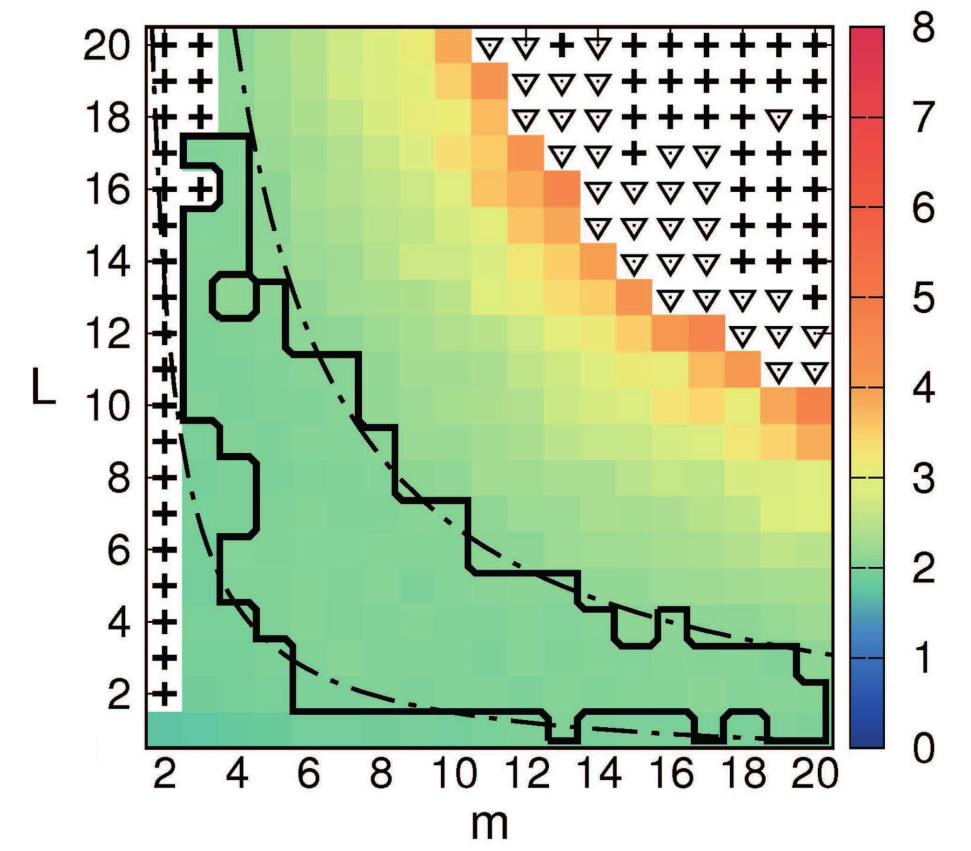
\includegraphics[width=.6\linewidth]{images/heatmap_Lorenz.png}
\caption{Correlation dimension of a Lorenz sequence as a function of the embedding parameters, using an embedding lattice
$[2, 20]\times[1, 20]$. Embedding pairs marked with a ``$+$'' sign provide incompatibility with the
requirement $\nu \leq m \leq \tau_I/(LT)$. Black triangles correspond to embedding pairs for which
an evaluation of $\nu$ is unavailable due to the algorithm exceeding the computational time limit.
The black solid line encompasses the lattice region corresponding to $\nu=2.05\pm0.05$.
The black dash-dotted curves are two hyperbolae bounding the region of uniform $\nu$ and
are defined by $(m-1)LT=0.4$ and $(m-1)LT=1.8$.
Figure adapted from Ref.~\cite{ref:perinelli2020chasing}.
}
\label{fig: Lorenz heatmap}
\end{figure}

\begin{figure}[h!]
    \centering
    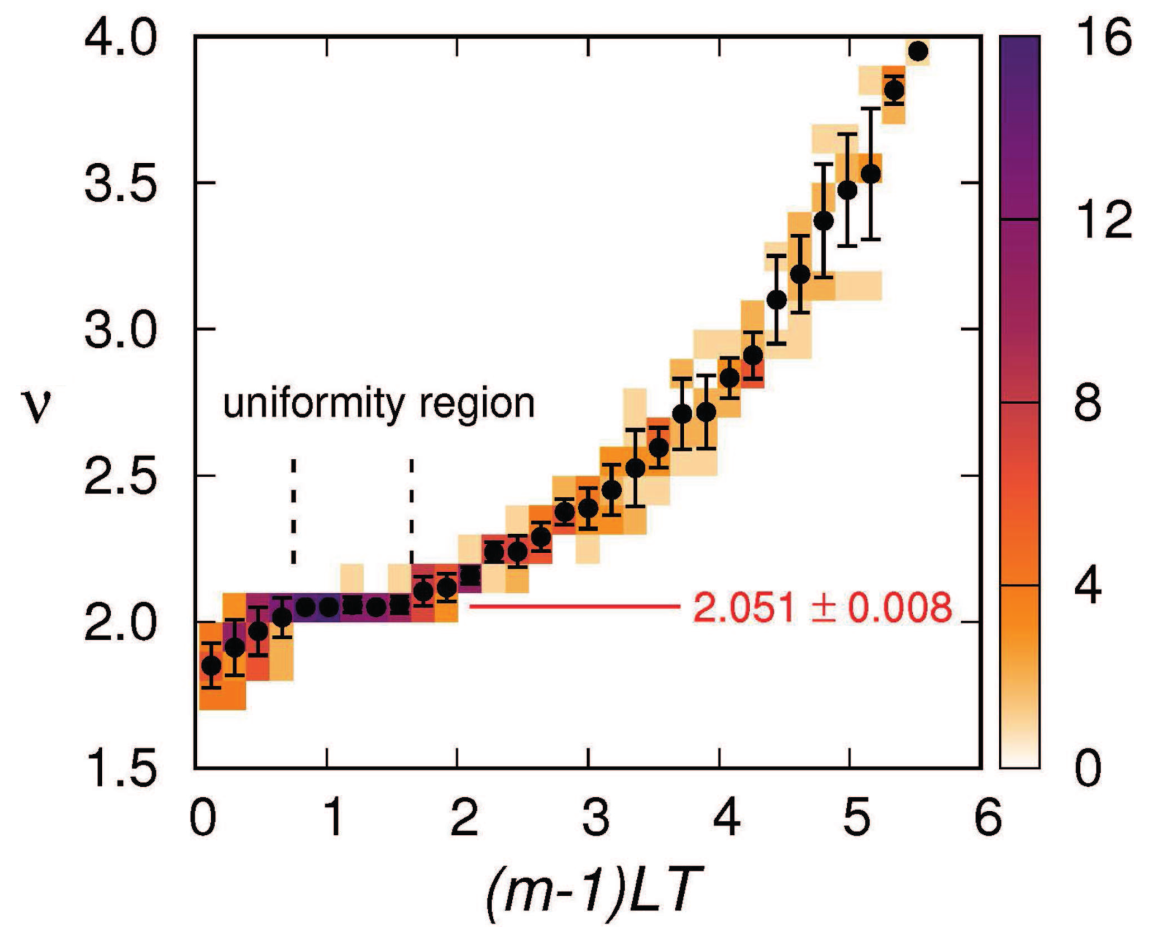
\includegraphics[width=.6\linewidth]{images/joint_Lorenz.png}
    \caption{Sample joint distribution of the correlation dimension $\nu$ as a function of the
    embedding window $(m-1)LT$ for the Lorenz sequence. Bin width is $0.1$ along the $\nu$ axis and
    $0.18$ along the $(m-1)LT$ axis.
    Black dots and the related errobars correspond to the expected value and the related uncertainty of
    $\nu$ for each given value (bin) of the embedding window. A uniformity region can be identified
    corresponding to embedding windows between $0.75$ and $1.65$. Averaging $\nu$ within
    the uniformity region yields $2.051 \pm 0.008$.
    Figure adapted from Ref.~\cite{ref:perinelli2020chasing}.
    }
    \label{fig: Lorenz joint}
\end{figure}

The robustness of this approach can be furtherly tested by affecting the Lorenz sequence with
observational noise. The elements $s_n$ of a noise-affected input sequence are given by
\begin{equation}
    \label{eq: noise sequence}
    s_n=x_n+\eta_n,
\end{equation}
where $x_n$ are the elements of the Lorenz sequence, and $\eta_n$ are independent
identically distributed random variables, which are distributed according to a normal distribution
with zero mean and variance $\sigma_\eta^2$.
The signal-to-noise-ratio (SNR) of a sequence is then defined as:
\begin{equation}
    \label{eq: snr}
    \text{SNR}= 20~\text{dB}~\log_{10}\left(\frac{\sigma_x}{\sigma_\eta}\right),
\end{equation}
where $\sigma_x=7.93$ is the standard deviation of the Lorenz sequence used in~\cite{ref:perinelli2020chasing}.

The sample joint distributions of the Lorenz sequence contaminated by noise are shown in Fig.
\ref{fig: Lorenz noise joint} for SNR equal to 30 dB (a), 20 dB (b) and 10 dB (c).
The uniformity region can only be identified in the 30 dB case, although the corresponding estimated
correlation dimension $\nu$ is about $15\%$ higher with respect to the noiseless case.

\begin{figure}[h!]
    \centering
    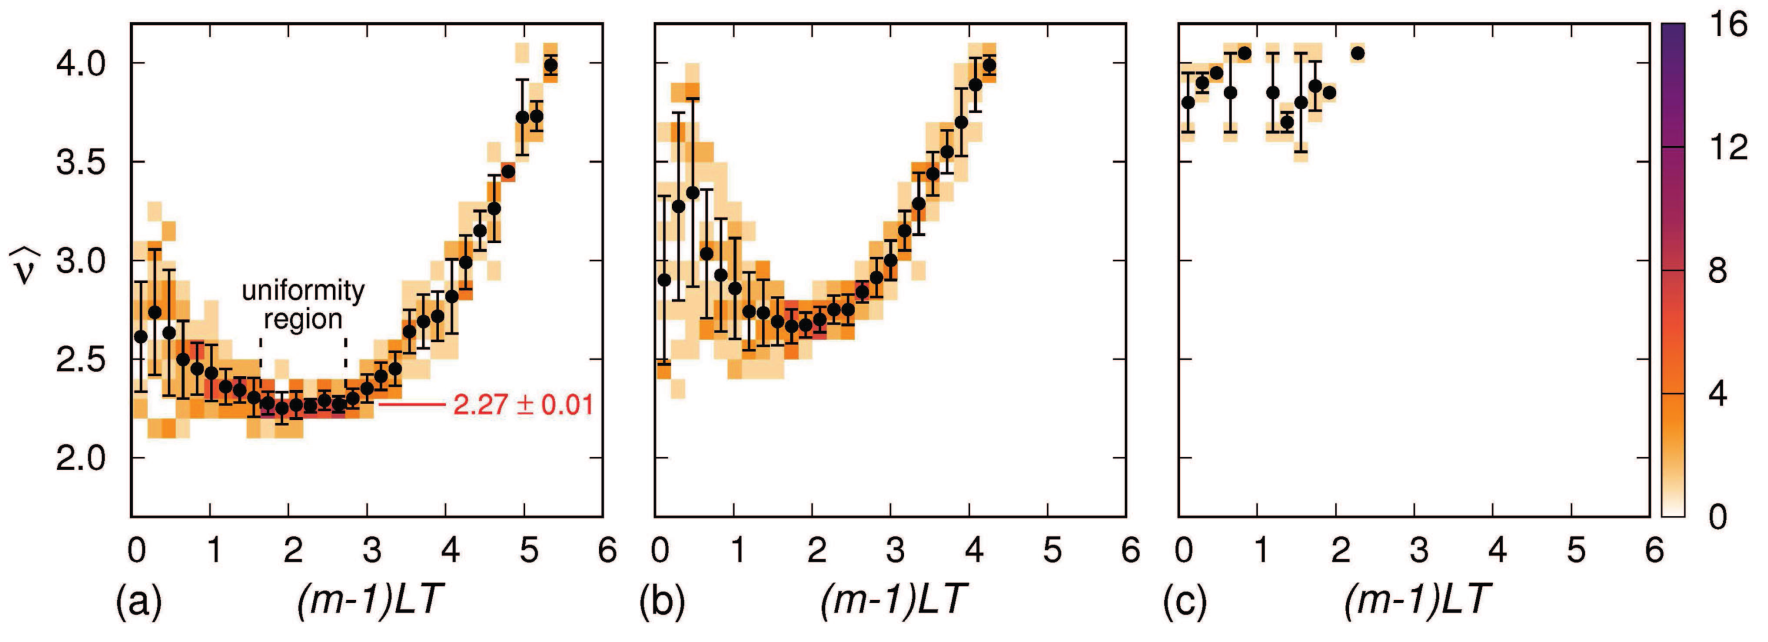
\includegraphics[width=\linewidth]{images/joint_Lorenz_noise.png}
    \caption{Sample joint distribution of the correlation dimension $\nu$ as a function of the
    embedding window $(m-1)LT$ for the Lorenz sequence contaminated by noise.
    SNR are equal to 30 dB (a), 20 dB (b) and 10 dB (c).
    Bin width is $0.1$ along the $\nu$ axis and
    $0.18$ along the $(m-1)LT$ axis.
    Black dots and the related errobars correspond to the expected value and the related uncertainty of
    $\nu$ for each given value (bin) of the embedding window. A uniformity region can be identified
    only in the case in which $\text{SNR}=30~\text{dB}$.
    Figure adapted from Ref.~\cite{ref:perinelli2020chasing}.
    }
    \label{fig: Lorenz noise joint}
\end{figure}

In conclusion, the method described in Section~\ref{sec: method for chaos} seems able to correctly identify
chaotic sequences even in presence of noise, provided that the signal to noise ratio is not too large.
In Chapter~\ref{chap: chaos analysis} this approach will be furtherly tested on the electronic implementation
of the Burridge-Knopoff model.

